\documentclass{article}

\usepackage{indentfirst}
\usepackage{scrextend}
\usepackage{changepage}
\usepackage{array,multirow}
\usepackage{graphicx}
\newcolumntype{L}[1]{>{\raggedright\let\newline\\\arraybackslash\hspace{0pt}}m{#1}}
\newcolumntype{C}[1]{>{\centering\let\newline\\\arraybackslash\hspace{0pt}}m{#1}}
\newcolumntype{R}[1]{>{\raggedleft\let\newline\\\arraybackslash\hspace{0pt}}m{#1}}

\begin{document}

\begin{titlepage}
	\title{Gerrymander Application: System Requirements}
	\author{Hyreus LTD.}
	\date{October 19, 2017}
	\maketitle
	\thispagestyle{empty}
\end{titlepage}



\tableofcontents
\thispagestyle{empty}
\cleardoublepage

\setcounter{page}{1}


%%%% Introduction %%%%

\section{Introduction}\label{sec:intro}

%%%% Purpose of This Document %%%%

\subsection{Purpose of This Document}

\vspace{2.5mm}

\begin{addmargin}[4em]{0em}

The purpose of this Systems Requirements document is to be used as a guideline throughout the development of the application. It will list the functional and non-functional requirements of this application and provide detailed information for each requirement. This document will also contain a User Interface section that details the front-end creation of the application. Each deliverable will be listed along with a due date for its submission. Lastly, any open issues will be listed. These issues will be further investigated and discussed as the development process progresses.

\end{addmargin}

\vspace{2.5mm}

%%%% References %%%%

\subsection{References}

\vspace{2.5mm}

\begin{addmargin}[4em]{0em}

[Enter References Here]

\end{addmargin}

\vspace{2.5mm}

%%%% Purpose of the Product %%%%

\subsection{Purpose of the Product}

\vspace{2.5mm}

\begin{addmargin}[4em]{0em}

Since the founding of the United States, gerrymandering has been used in order to strengthen one party's chance at winning an election. By splitting up voting districts strategically, parties skew the political landscape of their specific state, giving them an advantage. In a hypothetical situation, the districts would be divided in a way that portrays the actual data collected on registered voters. This program will provide the user with a way to see this hypothetical situation as well as create their own imbalances based on the percentages of party dominance they desire.

\vspace{2.5mm}

\end{addmargin}

%%%% Product Scope %%%%

\subsection{Product Scope}

\vspace{2.5mm}

\begin{addmargin}[4em]{0em}

This application will be connected to a database that will contain voter information for the state of Maryland. The database will be created to allow room for more states to be added, but we will be specifically be focusing on the state of Maryland. Using research on gerrymandering, we will use Python coding not only to efficiently gerrymander a state, but also to display it on Google Earth. Once displayed, the user will be given the option to use 2 sliders that will greatly effect the gerrymander display. The first slider will decide whether the user wants the map to be more or less gerrymandered. The second slider will decide whether you want the gerrymander to favor republicans or democrats. 

\end{addmargin}

\vspace{2.5mm}

%%%% Functional Requirements %%%%

\section{Functional Requirements}\label{sec:functionalReq}

\vspace{2.5mm}

\begin{addmargin}[4em]{0em}


\begin{center}
\hspace*{-2cm}      
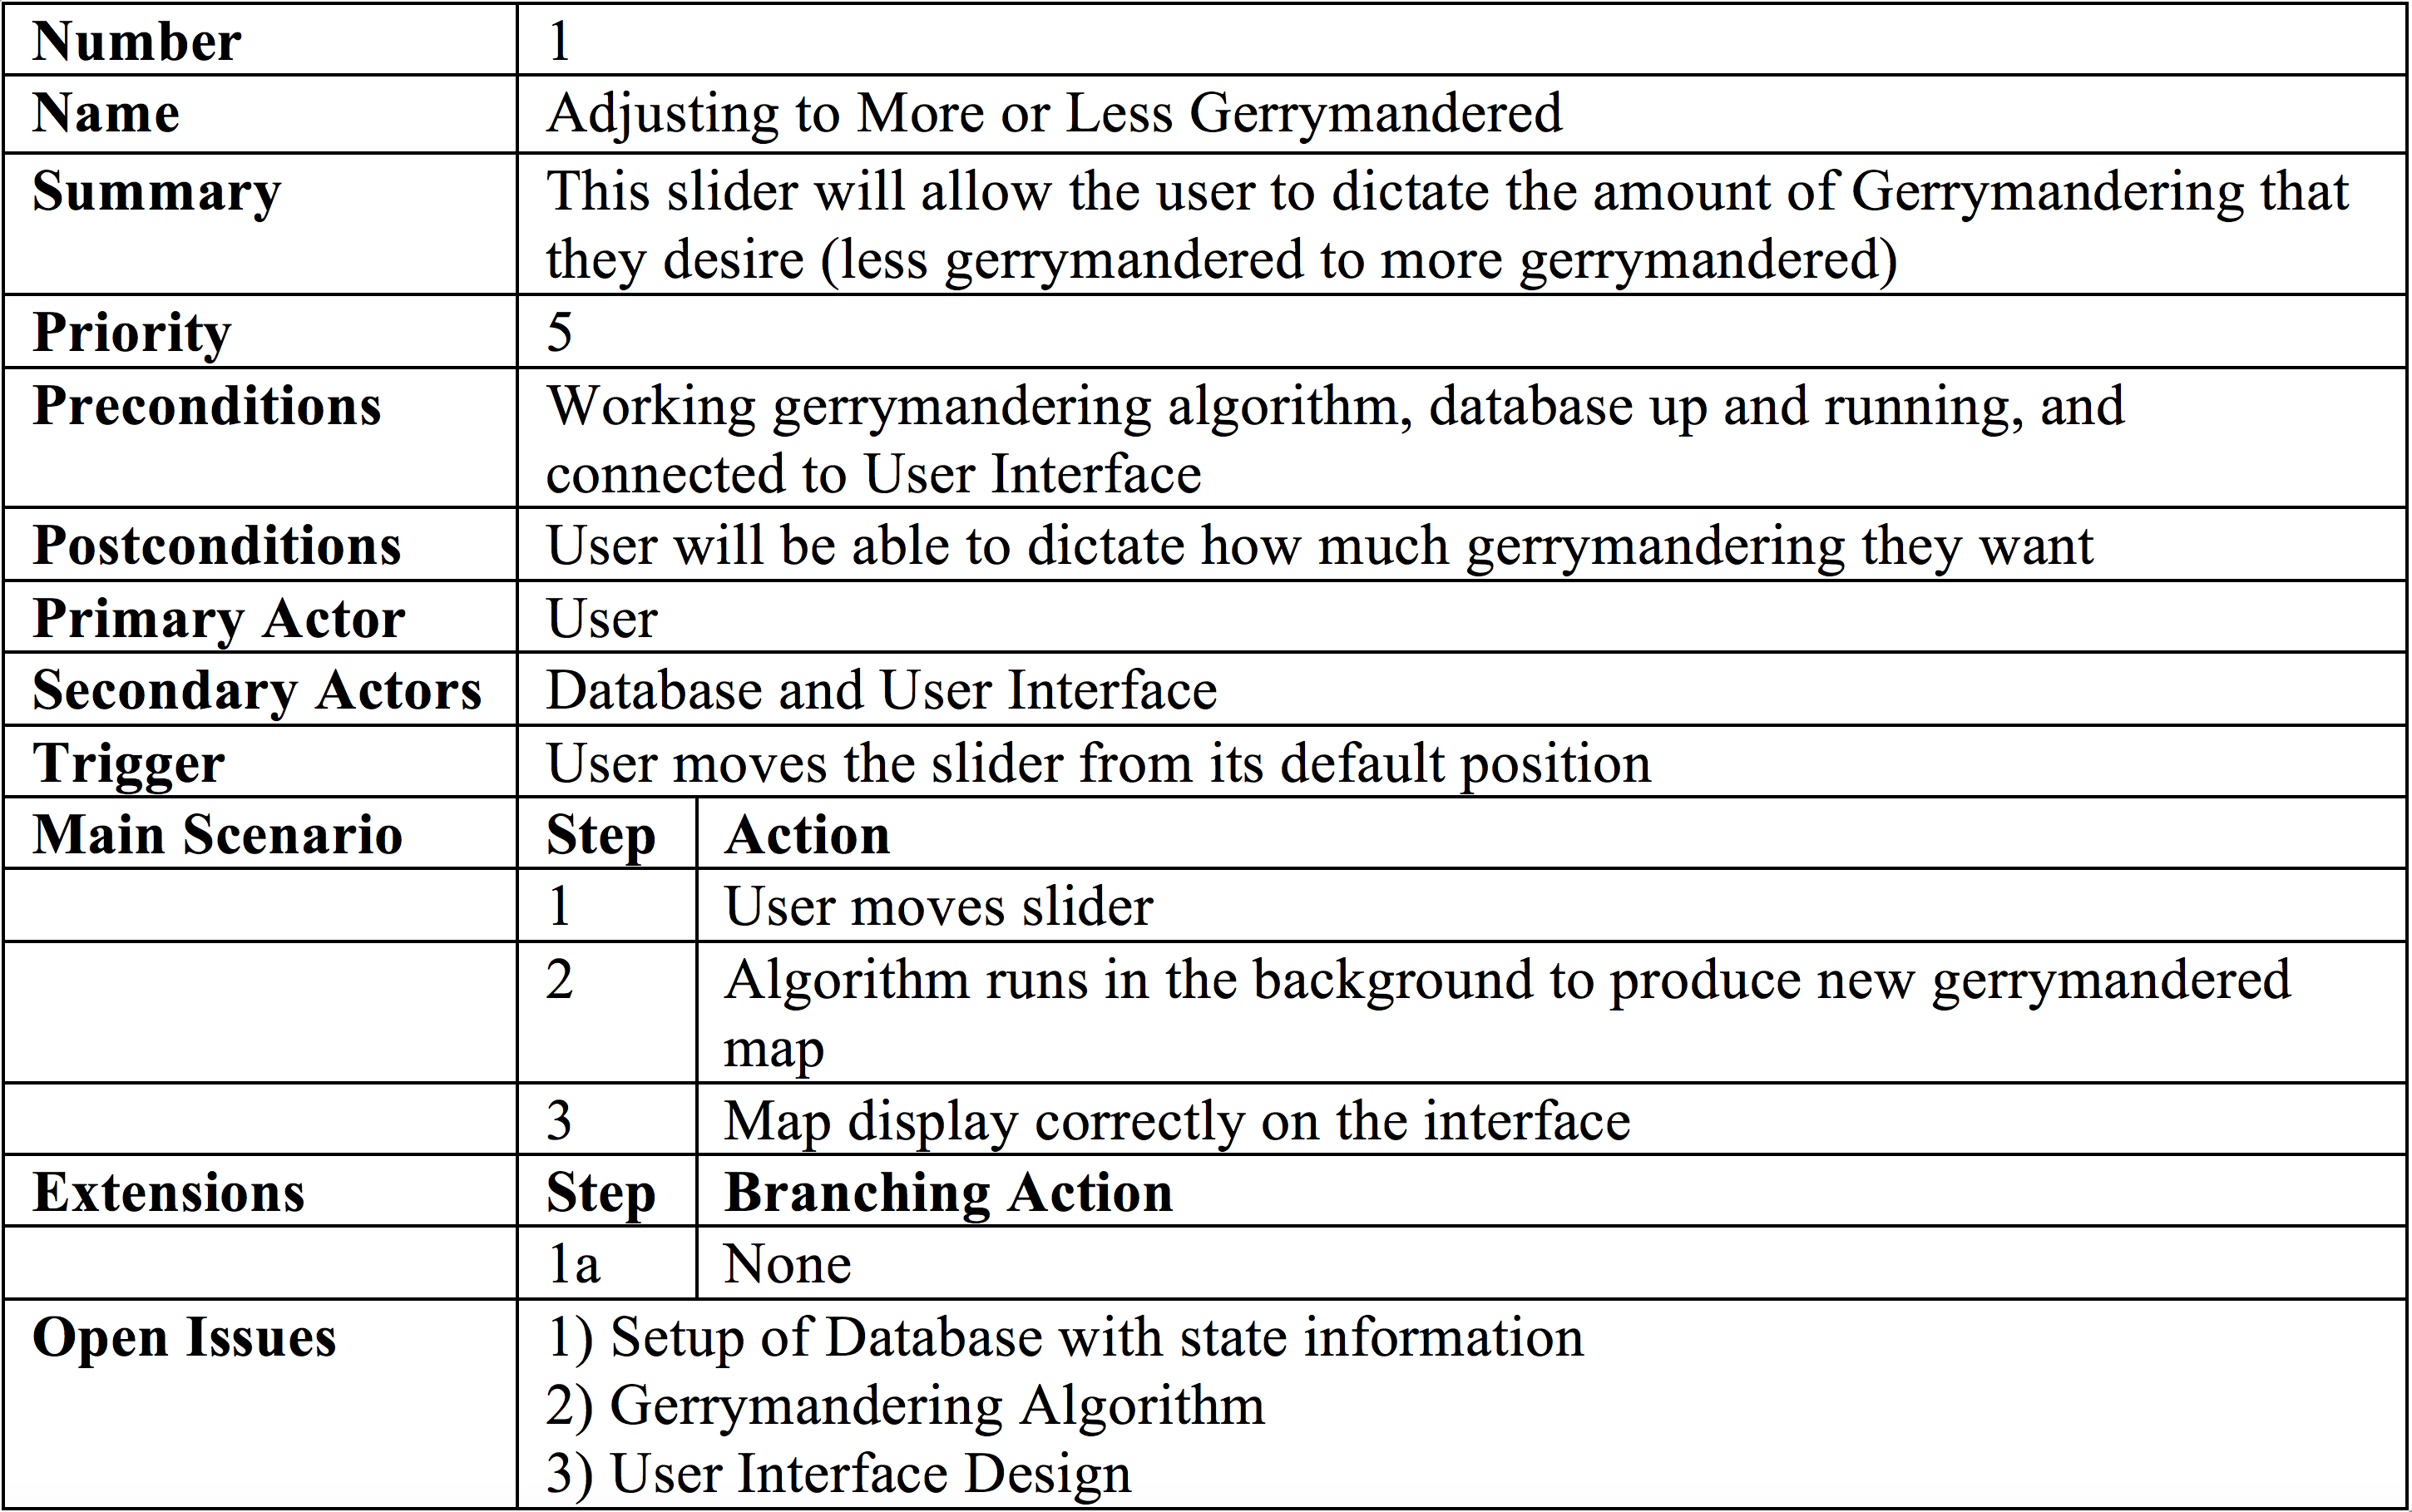
\includegraphics[scale=.8]{Slider1.png}
\end{center}



\begin{center}
\hspace*{-2cm}      
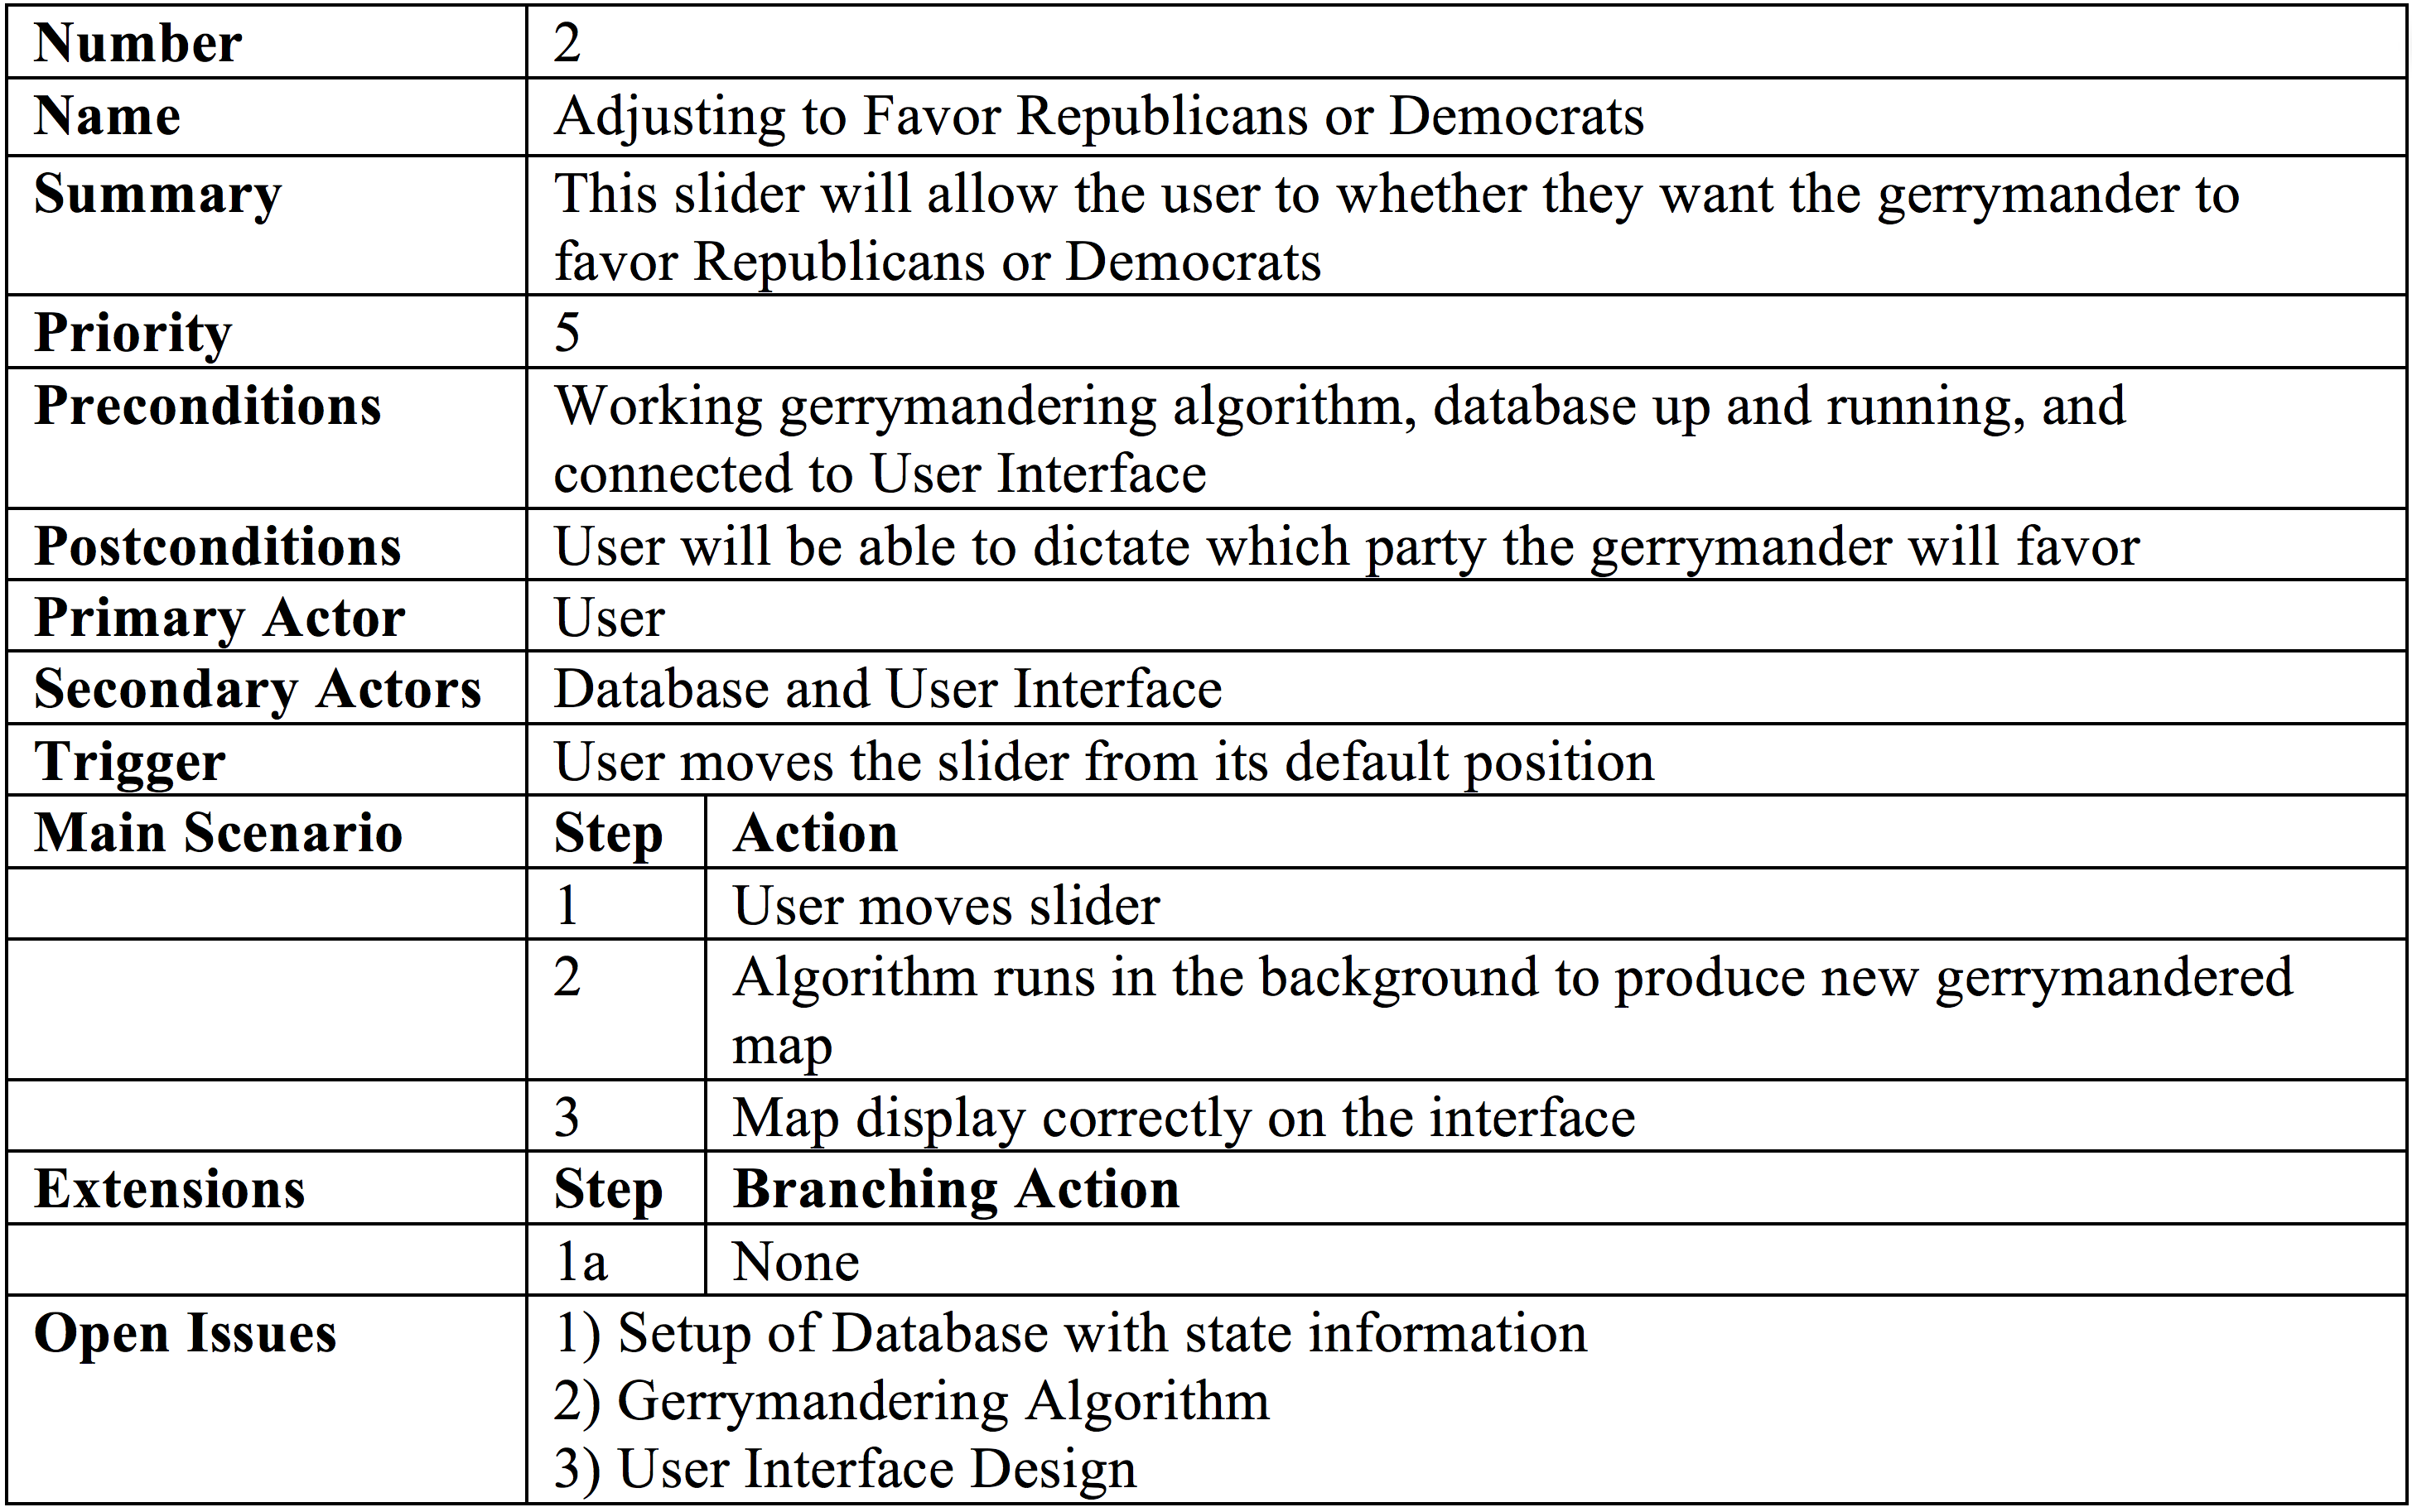
\includegraphics[scale=.8]{Slider2.png}
\end{center}


%\begin{table}[h]
%\centering
%\setlength\tabcolsep{3pt}
%\setlength\extrarowheight{2pt}

%\begin{tabular}{| l |  L{6cm}  L{5cm} |}
%\hline
%	Number &  1 & \\ \hline
%	Name &  Slider & \\ \hline
%	Summary &  This slider &   \\ \hline
%	Priority &  5  &\\ \hline
%	Preconditions &  Must have gerrymandering algorithm working  & \\ \hline
%	Postconditions &  User will be able to determine amount of gerrymandering  &  \\ \hline
%	Primary Actor &  User &  \\ \hline
%	Secondary Actors &  Database and User Interface & \\ \hline
%		Main Scenario: & \multicolumn{1}{ c | }{Step} & Actions \\ \hline 
%		& \multicolumn{1}{ l | }{1} & 'steps of use case from trigger to goal' \\ \hline 
%		& \multicolumn{1}{ l | }{2} & 'steps of use case from trigger to goal' \\ \hline 
%		& \multicolumn{1}{ l | }{3} & 'steps of use case from trigger to goal' \\ \hline 
		
%		Extensions: & \multicolumn{1}{ c | }{Step} & Branching Action \\ \hline 
%		& \multicolumn{1}{ l | }{1a} & 'condition causing branching' \\ \hline 
%		& \multicolumn{1}{ l | }{1b} & 'condition causing branching' \\ \hline 
%		& \multicolumn{1}{ l | }{1c} & 'condition causing branching' \\ \hline 
		%& 1) blah 1 & jjj \  \\ \hline
		%& 2) blah 2 & jjj \  \\ \hline
		%& 3) blah 3 & jjj \  \\ \hline

%	Open Issues & Open issues go here &  \\ \hline
%\end{tabular}
%\end{table}

%\begin{table}
%\centering
%\caption{Functional Requirement : Example 1}

%\begin{tabular}{ | r | r |} \hline
%Number & 1 \\ \hline
%Name & Name1 \\ \hline
%Summary & QuickDescription \\ \hline
%Priority & 1-5 \\ \hline
%Preconditions & PreCond. \\ \hline
%Postconditions & PostCond. \\ \hline
%Primary Actor & Actor1 \\ \hline
%Secondary Actors & Actors etc \\ \hline

%\end{tabular}
%\end{table}

\end{addmargin}

\vspace{2.5mm}

%%%% Non-Functional Requirements %%%%

\section{Non-Functional Requirements}\label{sec:non-functionalReq}

\vspace{2.5mm}

\begin{addmargin}[2em]{0em}
\begin{enumerate}

\item Response Time : The application should be able to give a response to the user's input within 400-500ms. The NFR rating is a 5. We will test this by running our animation in concert with a python clock package to test how fast the algorithm runs as well as how fast the display appears.

\item Effectiveness : The performance of our algorithms will produce accurate results in a timely manner. The results will be displayed correctly on the application with the use of sliders. There will be extensive research done on the best algorithms, and using the results of this research, we will come up with the best way to decide how to gerrymander a region. The NFR rating is a 5.

\item Documentation : With each paper requirement needed, it will be reviewed by the team and the customer before being pushed to our shared GitHub repository. Once pushed to the repository, we will submit the documents officially on blackboard as well as emailing the documents to the customer. The NFR rating is a 4. 

\item Reliability : The application should to withstand rapid changes to the sliders by the users while being able to display the correct data corresponding to those changes. Crashes should be handled gracefully. This NFR rating is a 4. We will test this by stress testing the database as well as finding beta users to test the user interface.

\item Scalability : While our main focus is the state of Maryland, the application should provide the ability to add additional states and be able to run the same algorithms on those added areas. The NFR rating is a 3. We will test this by testing the database and application with additional states.

\item Usability : The application will be not only efficient as far as showing the user how to effectively gerrymander a state, but also be educational. User's will find it easy to use the sliders and understand what they are affecting. The NFR rating is a 3. We will test this by doing beta testing and using the feedback to better our project. 

\item Transparency : There will be an open dialogue weekly with the customer where problems are discussed as well as progress made on whichever action has been assigned. The NFR rating is a 3. If the point of contact for our group can't physically make the meeting, an email will be sent with all of the information that would be discussed in the "in-person" meeting.

\item Quality : Code written should lead to no fatal errors. The code will be written under camelCase coding standards, as well as using tabs. The NFR rating is a 2.

\item Readability : While the code will be written by six people, it will look seamless as if one person wrote it. There will be consistent coding standards throughout as well as useful comments. The NFR rating is a 2.

\item Security : In our case security will not be as big of a focus, since there will be no personally identifiable information released, as well as this is a very small scale project. The NFR rating is a 1.

\end{enumerate}
\end{addmargin}

%%%% User Interface %%%%

\section{User Interface}\label{sec:ui}
\vspace{2.5mm}

See the User Interface Design Document for the Gerrymandering Application.

%%%% Deliverables %%%%
\vspace{2.5mm}
\section{Deliverables}\label{sec:deliverables}

Hard copies of each of the following:

\vspace{2.5mm}

\begin{adjustwidth}{2em}{0pt}
\begin{itemize}

\item Systems Requirement Specification (Due October 19)
\item System Design Document (Due October 26)
\item User Interface Design Document (Due October 26)
\item User Manual (Due November 30)
\item Administrator Manual (Due December 5)
\item Copies of all Biweekly Status Reports (Bi-Weekly)

\end{itemize}
\end{adjustwidth}

\vspace{5mm}

An electronic file containing the following: 

\vspace{2.5mm}

\begin{adjustwidth}{2em}{0pt}
\begin{itemize}

\item Systems Requirement Specification (Due October 19)
\item System Design Document (Due October 26)
\item User Interface Design Document (Due October 26)
\item User Manual (Due November 30)
\item Administrator Manual (Due December 5)
\item All source code (Due December 12)
\item The executable program (Due December 12)
\item Any other software required for installation and execution of the delivered program (Due December 12)

\end{itemize}
\end{adjustwidth}

%%%% Open Issues %%%%

\section{Open Issues}\label{sec:openIssues}

\vspace{2.5mm}

\begin{addmargin}[2em]{0em}

\begin{enumerate}

\item The specific details on the gerrymandering algorithm (equations, run time, etc...).
\item The collection and analysis of the voter census data.
\item Specifics on the aesthetics of the user interface.
\item Whether or not to have a backup for the database, and if so how that will be implemented.
\item The number of fields for each table in the database.

\end{enumerate}
\end{addmargin}

%%%% Appendix %%%%

\section{Appendix A - Agreement Between Customer and Contractor}\label{sec:apendixA}

\vspace{2.5mm}

\begin{addmargin}[2em]{0em}

See attached document.

\end{addmargin}

\section{Appendix B - Team Review Sign-Off}\label{sec:appendixB}

\vspace{2.5mm}

\begin{addmargin}[2em]{0em}

There are no comments as there were no disagreements. See attached document.

\end{addmargin}

\section{Appendix C - Document Contributions}\label{sec:appendixC}

\vspace{2.5mm}

\begin{addmargin}[2em]{0em}

\begin{enumerate}

\item Jamal Savoy : I took ownership over this document so a bulk of the document is my work. After learning LaTex, I created the outline and began filling it out with the information our team discussed with the customer at our first meeting. I worked on all of the sections and would estimate I did around 90\% of the document.

\item Austin DeLauney : 

\item Ben Kolarik : 

\item Brad Harmening : I reviewed the document and made the necessary spelling and grammatical adjustments.

\item Damien Overton : 

\item Dylan Demchuk : 

\end{enumerate}
\end{addmargin}


\end{document}